\documentclass{article}
\usepackage{adjustbox}
\usepackage{float}
\usepackage{textcomp}
\usepackage{graphicx}
\graphicspath{{images/}}
\usepackage{booktabs}
\usepackage{color}
\usepackage{verbatim}
\usepackage{listings}
\usepackage{underscore}
\setcounter{secnumdepth}{5}
\usepackage[bookmarks=true]{hyperref}
\author{Roberto Clapis (841859), Erica Stella (854443)} 
\date{\today}
\title{Politecnico di Milano
		\\A.A. 2015\@-\@2016
		\\Software Engineering 2: ``myTaxiService''
		\\\textbf{D}esign \textbf{D}ocument}
		\hypersetup{pdftitle={Design Document},    % title
		pdfauthor={Roberto Clapis, Erica Stella},                     % author
		pdfsubject={Design Document},                        % subject of the document
		pdfkeywords={TeX, LaTeX, taxi, DD, SoftwareEngineering2}, % list of keywords
		colorlinks=true,       % false: boxed links; true: colored links
		linkcolor=black,       % color of internal links
		citecolor=blue,       % color of links to bibliography
		filecolor=black,        % color of file links
		urlcolor=purple,        % color of external links
}
\begin{document}
\maketitle
\begin{center}
	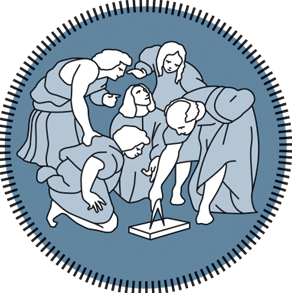
\includegraphics{polimi-logo}
\end{center}
\clearpage
\tableofcontents
\clearpage

\section{Introduction}
\subsection{Purpose}
The purpose of the Design Document is to provide documentation in order to aid the development of myTaxiService's system by providing a description of how it should be built and how its components are expected to interact with each other.
\subsection{Scope}
This Design Document is intended to explain the design and architecture of myTaxiService, a new application that will provide an easy way to access the taxi service in a city. It describes the system both from a software and hardware point of view, in order to clarify the system's structure and how it accomplishes its functionalities. 
\subsection{Definitions, Acronyms, Abbreviations}
\paragraph{Definitions}
\begin{itemize}
	\item \textit{End users:} this category comprises all those who use the application\footnotemark: administrators, taxi drivers, logged in users and guests.
\end{itemize}
\footnotetext{For their definition we refer to the RASD's section 1.6}
\paragraph{Acronyms}
\begin{itemize}
	\item \textit{UI:} user interface through which the end users can interact with the application.
	\item \textit{DB:} Database.
	\item \textit{DBMS:} Database Management System.
	\item \textit{SSL:} Secure Socket Layer, a protocol that ensures a safe end-to-end transmission.
\end{itemize}
\subsection{Reference Documents}
\begin{itemize}
	\item \href{run:./external_references/assignments.pdf}{Document} with the assignment for the project
	\item \href{run:./external_references/Rasd.pdf}{RASD} for myTaxiService
	\item \href{run:./external_references/DDTOC.pdf}{Template} for the Design Document
	\item \href{run:./external_references/IEEESoftwareDesignDescriptions.pdf}{IEEE standard} for Software Design Document
	\item The \href{run:./external_references/IEEEArchitectureDescription.pdf}{IEEE standard} for architecture descriptions
\end{itemize}
\subsection{Document Structure}
The following parts of this document are structured in 3 sections: architectural design, user interface design and requirements traceability. The architectural design section describes the software and hardware components of the system and their interactions. The user interface design section which refers to the ``User Interfaces'' subsection of the RASD\@. The requirements traceability section that explains how the proposed design meets the requirements that have been defined in the RASD\@.
\clearpage
\section{Architectural Design}
\subsection{Overview}
The system to be developed, as mentioned before, will be used to provide an easy access to a taxi service. Therefore, its main functionalities, that will have to be supported by the design and architecture, are: the storage of the taxi drivers' and clients' accounts, the computation of the taxi queue of each zone and the handling of requests and reservations. Furthermore, the system will have to comply to quality of service attributes as specified in the RASD\@.
\subsection{High Level Components and Their Interaction}
myTaxiService's system is composed by three main components: DBMS, Web Server and client application. The client application provides the UI through which end users can access the application's services. These requests are forwarded to the Web Server which is in charge of providing a response, eventually querying the Database in the DBMS for information. The Web Server is also responsible for answering to the API calls coming from external applications and notifying the end users for particular events, like when a request is accepted by a taxi driver. The DBMS stores all the information of the end users's accounts, the active requests and reservations.
\subsection{Component View}
%TODO aggiungere http interfaccia smista
\begin{figure}[H]
	  \makebox[\textwidth][c]{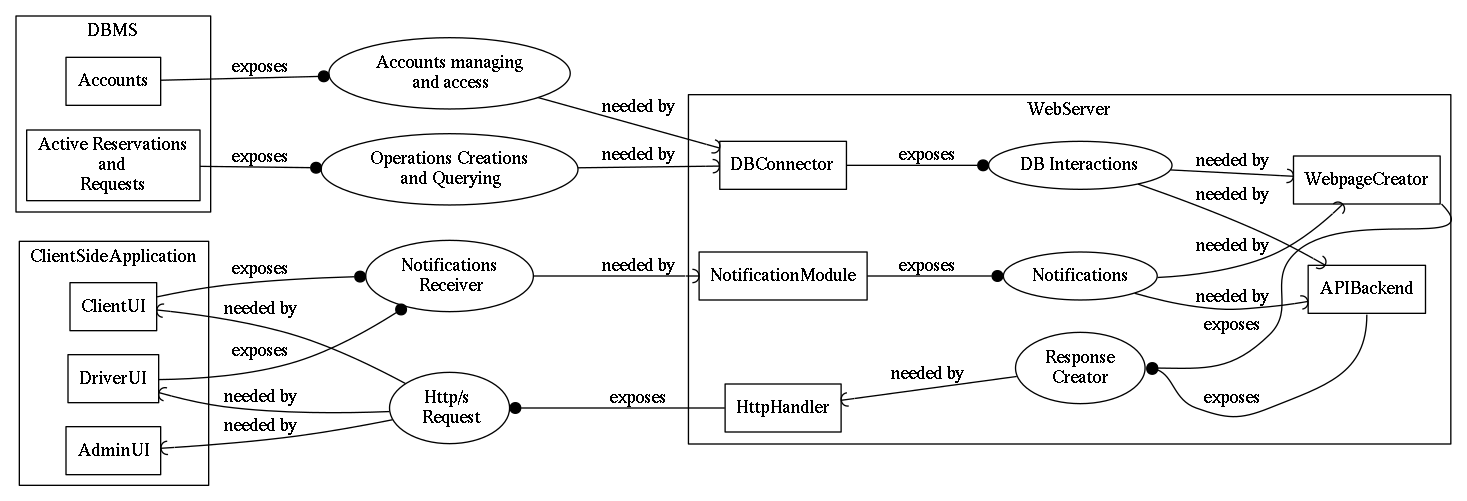
\includegraphics[width=1.4\textwidth]{Component}}%
\end{figure}
	  While the DBMS and the Client Side application are pretty much self explanatory the WebServer part requires some details:
	  \begin{itemize}
			  \item The Webpage Creator is the responsible for both the Mobile App and Web App responses. The httpHandler will recognize the request by the parameters and ask the Webpage Creator to either create the full HTML page (in the case of the Web App) or just send a partially created page that only contains the dynamic data that the Mobile App will then include in its interface.
			  \item The API Backend will be called by the httpHandler and will respond with Only the data requested in a JSON format
	  \end{itemize}
\subsection{Deployment View}
\begin{figure}[H]
	  \makebox[\textwidth][c]{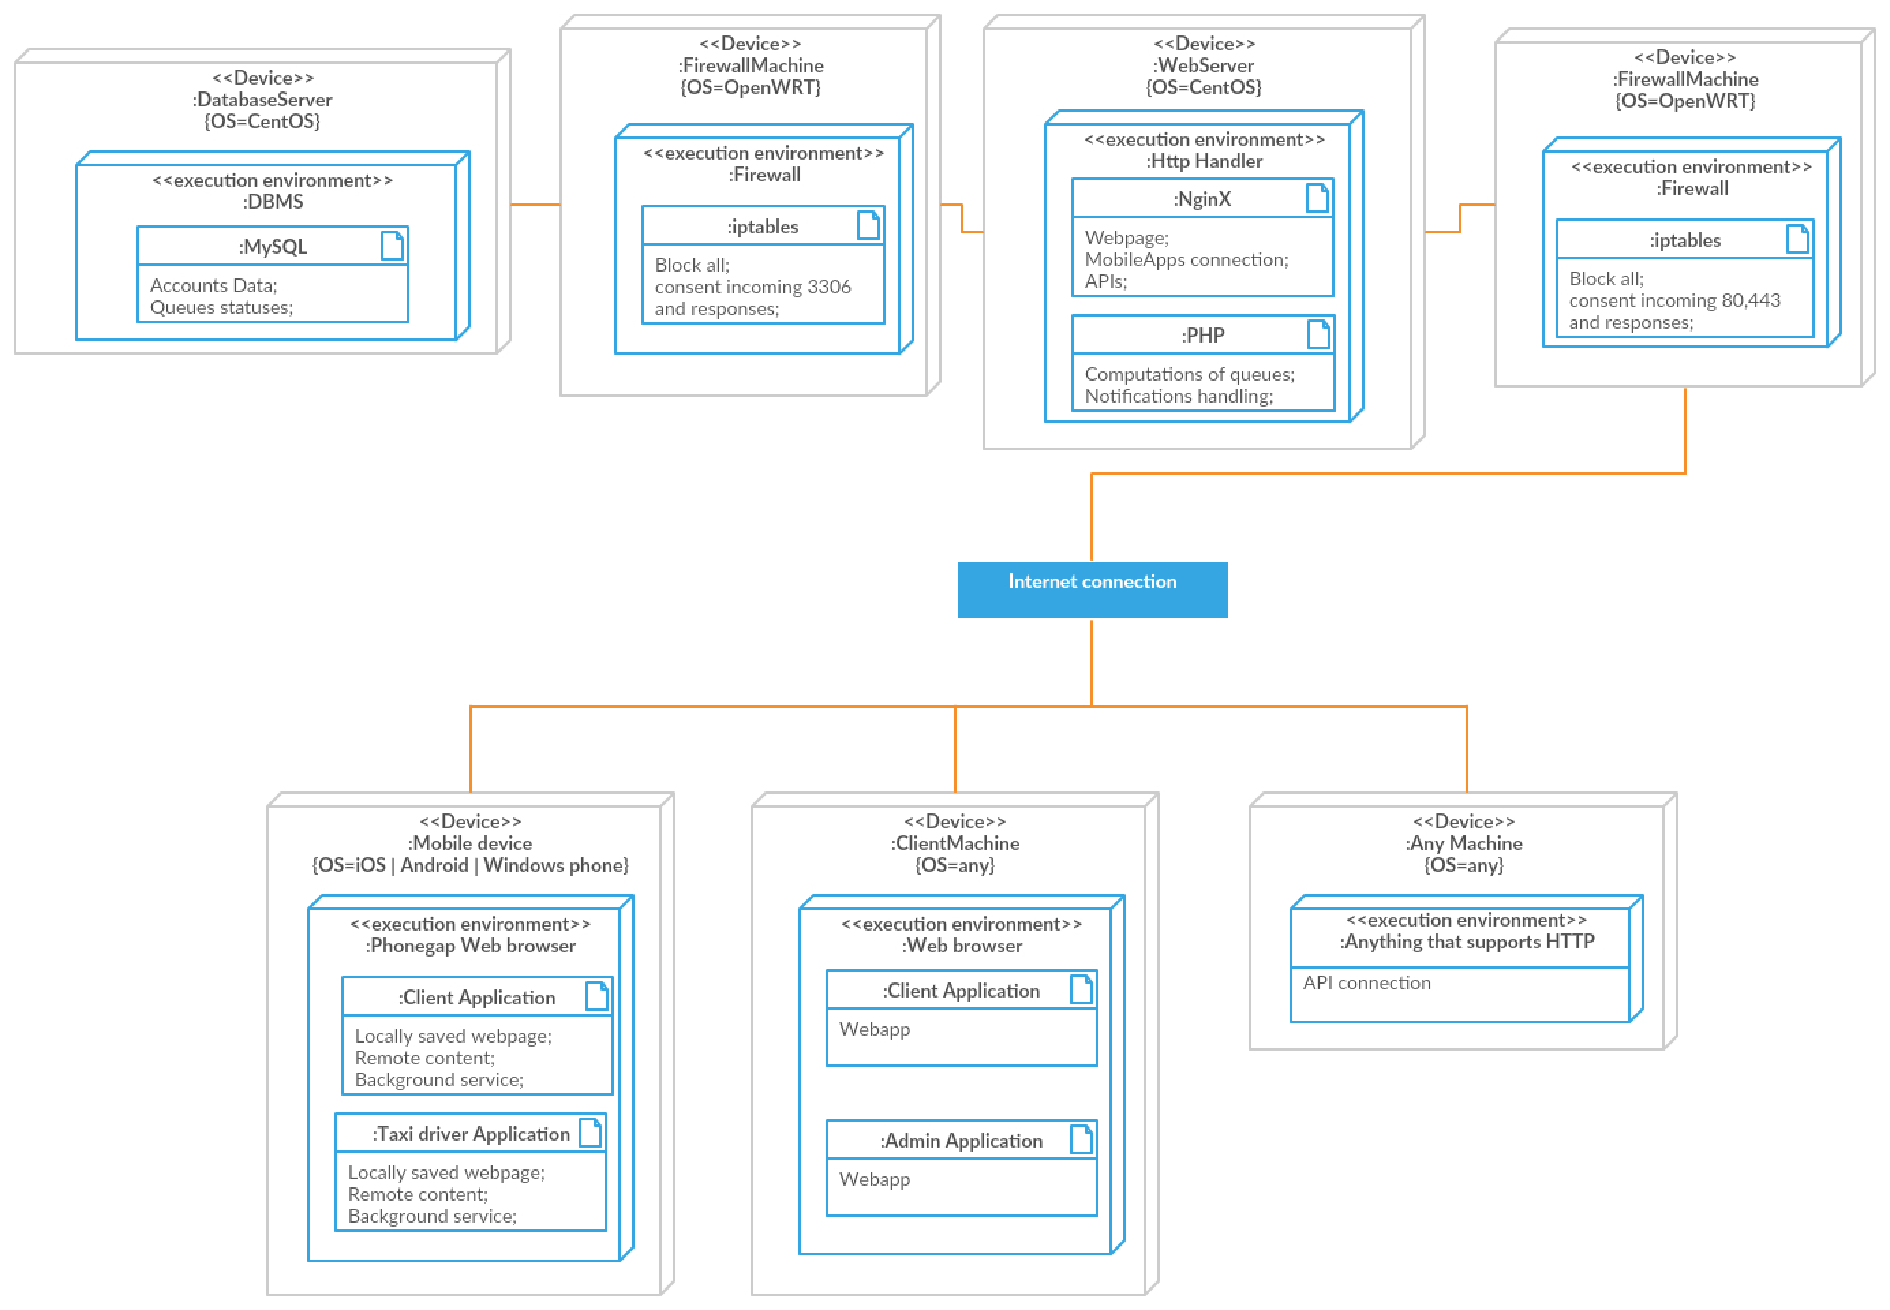
\includegraphics[width=1.3\textwidth]{Deployment}}%
\end{figure}
		This is just a pretty standard configuration with DMZ, Internal network, double firewall and untrusted network, see more in section 2.8
\subsection{Runtime View}

\begin{figure}[H]
	  \makebox[\textwidth][c]{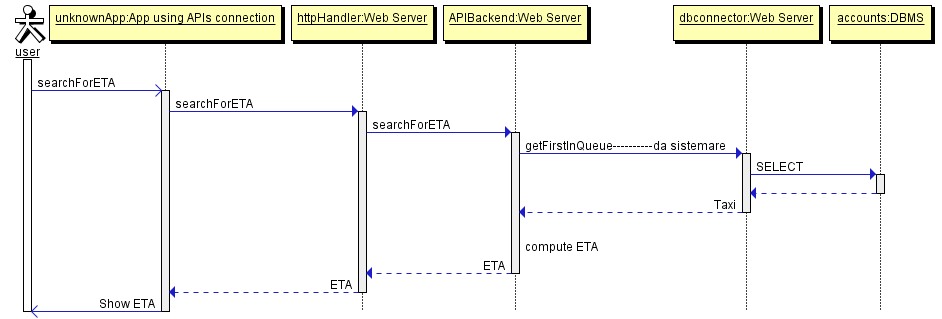
\includegraphics[width=1.3\textwidth]{sdedit/APIUsage.png}}%
\end{figure}
\begin{figure}[H]
	  \makebox[\textwidth][c]{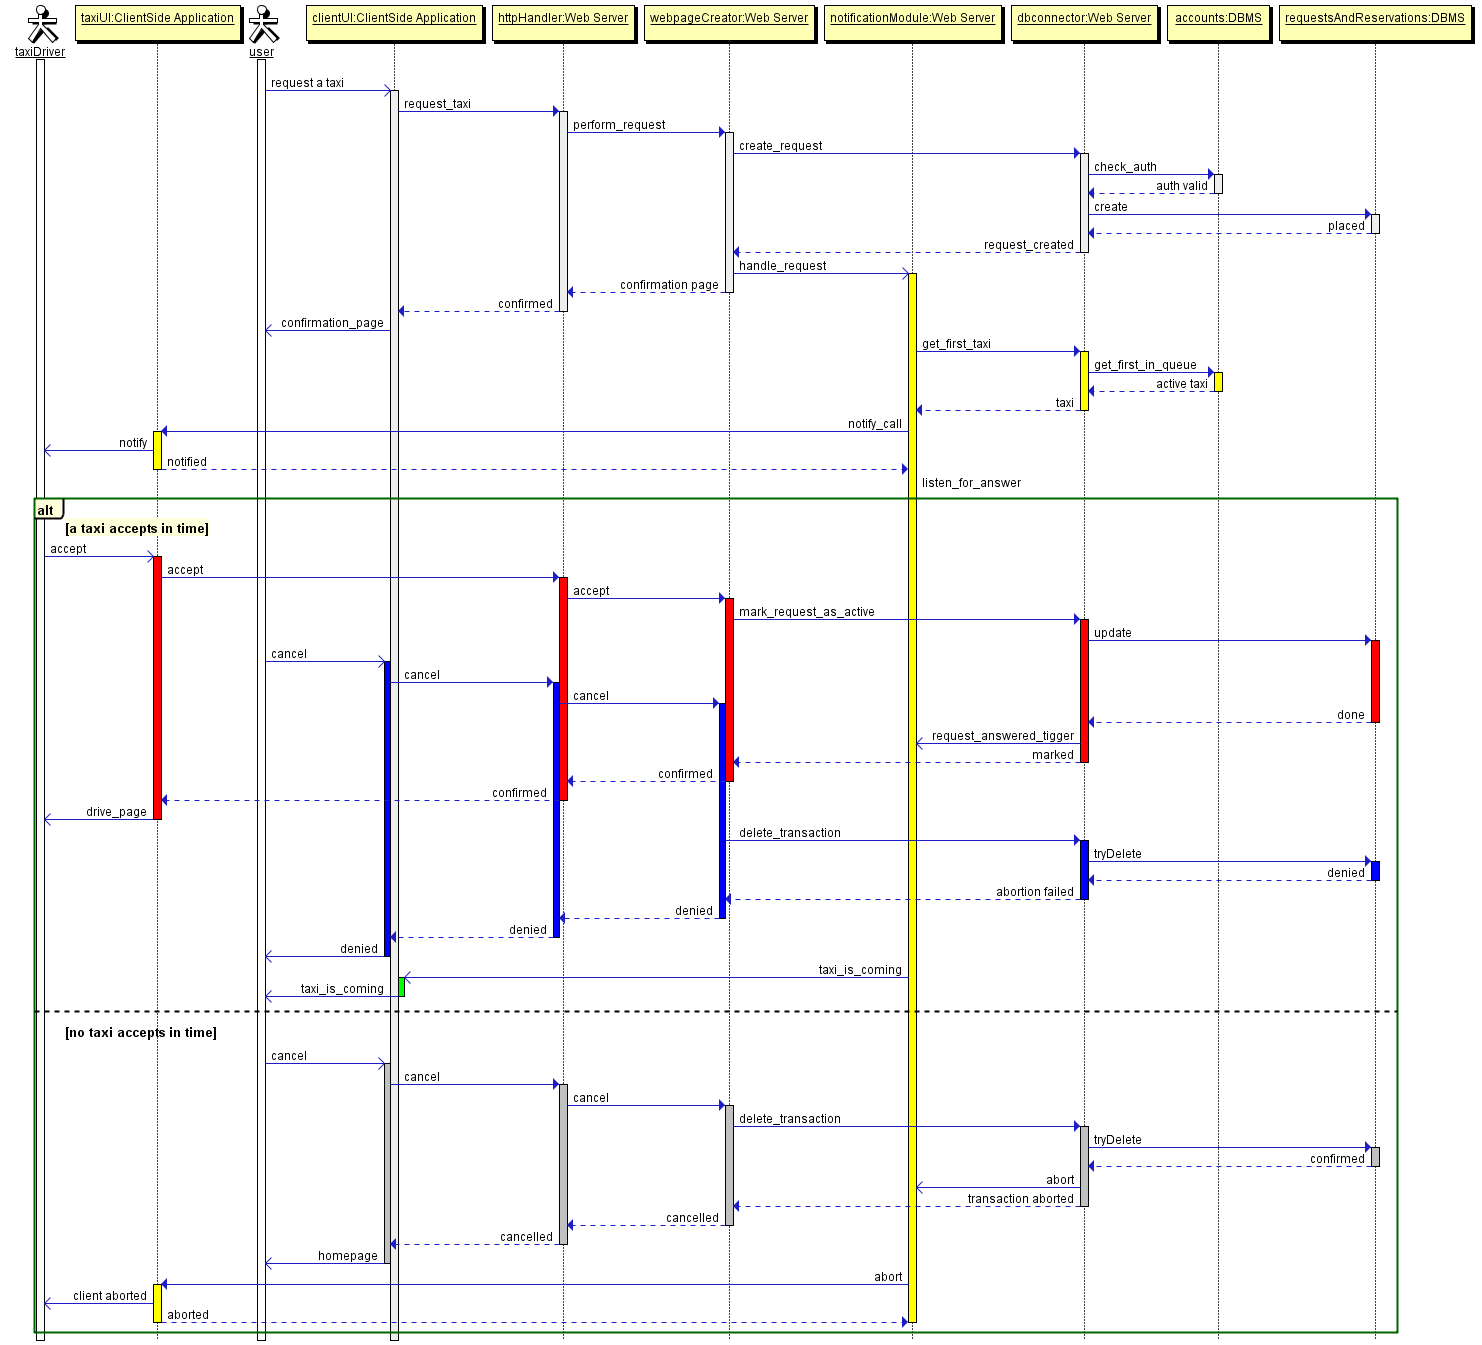
\includegraphics[width=1.3\textwidth]{sdedit/Cancel.png}}%
\end{figure}
\begin{figure}[H]
	  \makebox[\textwidth][c]{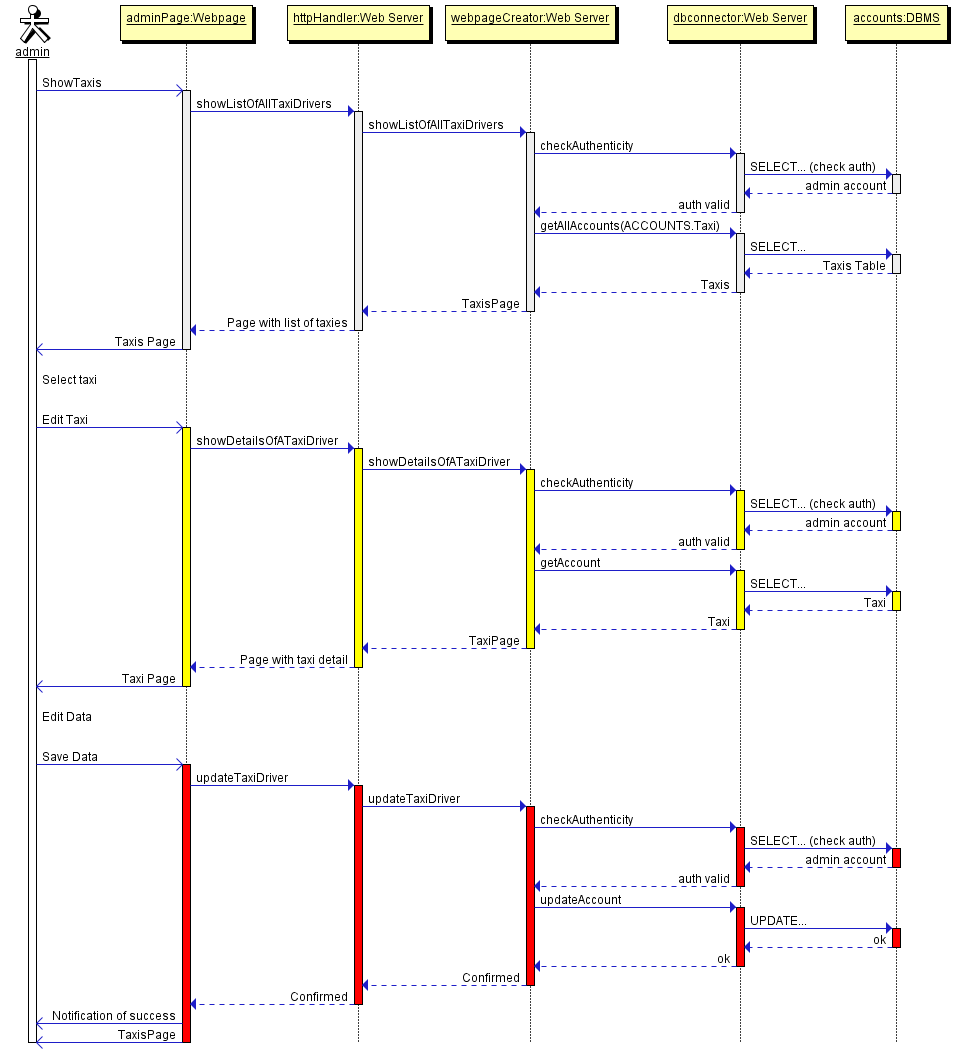
\includegraphics[width=1.3\textwidth]{sdedit/ChangeData.png}}%
\end{figure}
\begin{figure}[H]
	  \makebox[\textwidth][c]{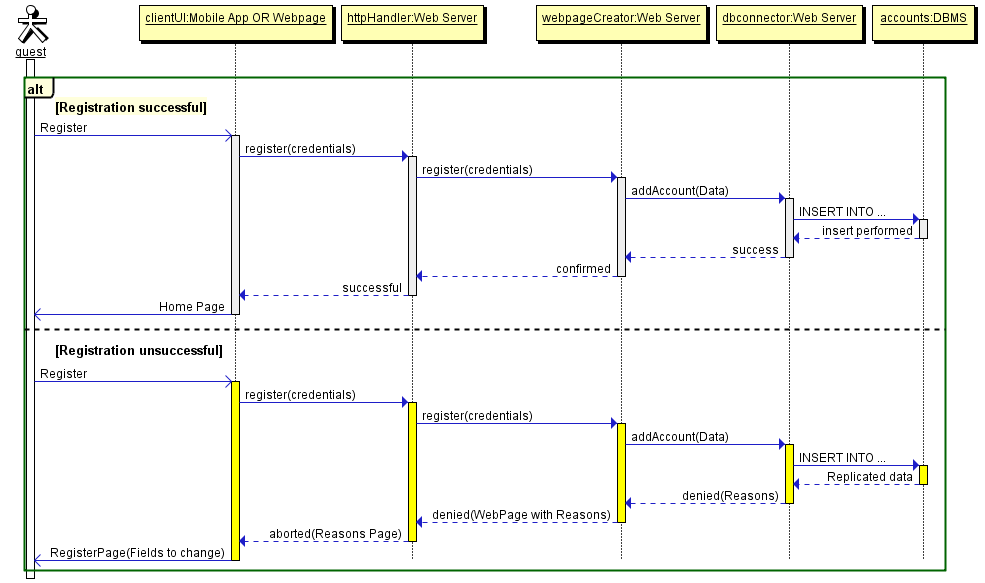
\includegraphics[width=1.3\textwidth]{sdedit/Registration.png}}%
\end{figure}
\begin{figure}[H]
	  \makebox[\textwidth][c]{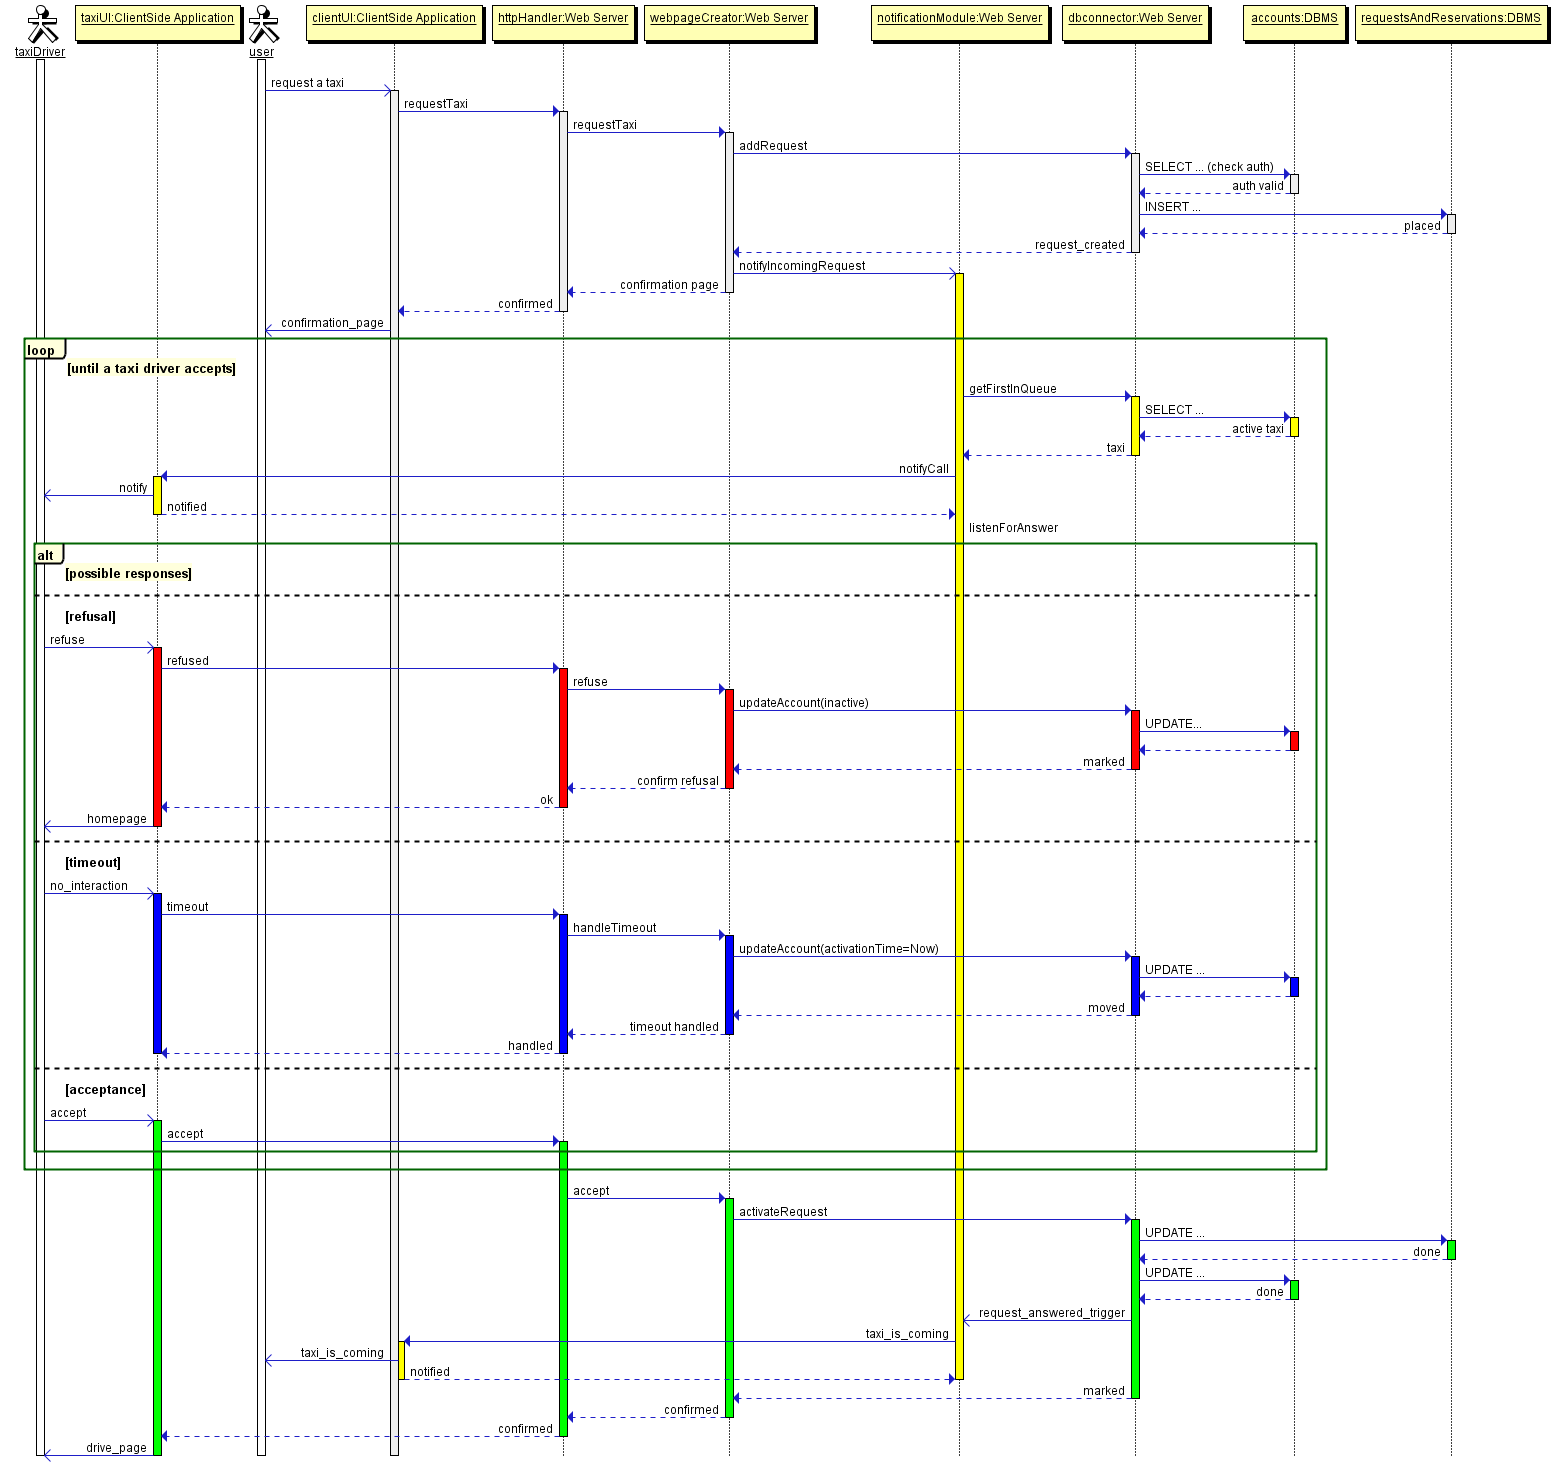
\includegraphics[width=1.3\textwidth]{sdedit/Request.png}}%
\end{figure}
Some details:
\begin{itemize}
	\item HTTPS negotiations are omitted in order to preserve readability, but they would all be between the apps (Web or Mobile)  and the httpHandler
	\item Queues are not represented in the database, but they are all re-computed with a query that selects the taxis that are active, are in the desired area and returns them sorted by the time they were marked as active.
\end{itemize}
%TODO sequence diagrams
\subsection{Component Interfaces}
\paragraph{DB Interactions}
This interface encapsulates and exposes all the operations the Web Server needs to interact with the DB\@. The operations are divided in 2 categories based on the DB's part they manage:
\begin{itemize}	
	\item \textit{Accounts managing and access:} this interface exposes methods to manage the stored end users accounts.\\	
	\begin{table}[H]
		\begin{adjustbox}{width=1.2\textwidth}
			\begin{tabular}{*{3}{c}}
				\toprule
				Method & Parameters required & Notes \\
				\midrule
				addAccount & account type and credentials & adds an account to the DB of the specified type if there's not another one with the same ID\\
				updateAccount & user ID, attribute to modify, and value & updates the attribute specified to the new value\\ 
				deleteAccount & user ID & deletes the account specified by the ID \\
				getAccount & user ID & returns the account corresponding to the ID with all its attributes \\
				getAllAccounts & type of the accounts & returns all the accounts of the specified type \\
				getFirstInQueue & location & returns the first taxi (by activation time) that is in the given location\\
				checkAuthenticity & user ID & returns true if the specified account is in the DB, false otherwise \\
				getFirstInQueue & starting location's zone & returns the first taxi driver of the queue of the specified zone \\
				\bottomrule
			\end{tabular}	
		\end{adjustbox}
	\end{table}
\item \textit{Operations creations and querying:} this interface exposes methods to manage and retrieve requests and reservations.\\	
	\begin{table}[H]
		\begin{adjustbox}{width=1.2\textwidth}
		\begin{tabular}{*{3}{c}}
			\toprule
			Method & Parameters required & Notes \\
			\midrule
			addRequest & starting location, destination, user ID & adds a new ``not accepted'' request to the DB from the user that requested it and returns its ID to the caller\\ 
			deleteRequest & request ID & deletes an existing request from the DB and returns true. If the request is marked as not removable it returns false\\ 
			activateRequest & request ID, taxi ID & changes the state of the request from ``not accepted'' to ``accepted'' and the taxi's state to unavailable. It also marks the request as not removable\\
			getRequest & request ID & returns the request specified by the ID and all its attributes\\
			getAllUserCalls& user ID & returns all the active requests and reservations of the specified user \\
			addReservation & starting locations, destination, meeting time & adds a new reservation to the DB from the specified user and return its ID\\
			deleteReservation & reservation ID & deletes an existing reservation from the DB and returns true. If the reservation is marked as not removable it returns false\\
			activateReservation & reservation ID, taxi ID & changes the state of the reservation from ``not accepted'' to ``accepted'' and the taxi to unavailable. It also marks the reservation as not removable\\
			getReservation & reservation ID & returns the reservation specified by the ID with all its attributes\\
			\bottomrule
		\end{tabular}	
	\end{adjustbox}
\end{table}
\end{itemize}

\paragraph{Response creator}
This interface exposes all the functionalities end users require to access the services offered by myTaxiService. 
In the following list the methods are divided by type of end user that needs them. 
\begin{itemize}
	\item \textit{Functionalities exploited by guests:}	\\
	\begin{table}[H]
		\begin{adjustbox}{width=1.2\textwidth}
			\begin{tabular}{*{3}{c}}
				\toprule
				Method & Parameters required & Notes \\
				\midrule
				searchForETA & starting location & returns the ETA\footnotemark\  of the CAT\footnotemark\\ %
				register & credentials & if the credentials don't refer to an already existing account, a new one is created \\
				login & credentials & the guest logs into the system \\
				\bottomrule
			\end{tabular}
	\end{adjustbox}
\end{table}
\footnotetext{See RASD's section 1.5.2}
\footnotetext{See RASD's section 1.5.2}

	\item In the following tables, user IDs are always passed as a parameter, as they are needed for the authentication, but they're omitted for readability. \\	

	\item \textit{Functionalities exploited by logged in user:} logged in user can access the searchForETA method exposed for guests along with the following methods: 
	\begin{table}[H]
		\begin{adjustbox}{width=1.2\textwidth}
			\begin{tabular}{*{3}{c}}
				\toprule
				Method & Parameters required & Notes \\
				\midrule
				requestTaxi & starting location, destination & requests a taxi for the specified starting location \\ 
				cancelRequest & request ID & cancels the request if it's not already been accepted\\ 
				showRequestDetails & request ID & shows the details of the specified request\\
				reserveTaxi & starting location, destination, meeting time & reserve a taxi for the specified starting location and meeting time \\
				cancelReservation & reservation ID & cancels the reservation if it's not already been accepted \\
				showReservationDetails & reservation ID & shows the details of the specified reservation\\
				logout &  & the user is logged out of the system \\
				\bottomrule
			\end{tabular}
		\end{adjustbox}
	\end{table}	
	\item \textit{Driver:}		
	\begin{table}[H]
		\begin{adjustbox}{width=1.2\textwidth}
			\begin{tabular}{*{3}{c}}
				\toprule
				Method & Parameters required & Notes \\
				\midrule
				accept & request or reservation ID & the request or reservation for which the taxi driver has been notified, specified by its ID, is accepted \\ 
				refuse & request or reservation ID & the request or reservation for which the taxi driver has been notified, specified by its ID, is refused\\ 
				toggleState & & the state of the taxi driver is changed from not available to available, or vice versa\\
				\bottomrule
			\end{tabular}
		\end{adjustbox}
	\end{table}		
	\item \textit{Admin:}
		\begin{adjustbox}{width=1.2\textwidth}	
			\begin{tabular}{*{3}{c}}
				\toprule
				Method & Parameters required & Notes \\
				\midrule
				addTaxiDriverAccount & credentials & a new account for a taxi driver is created with the specified credentials\\ 
				updateTaxiDriverAccount & attributes to update, new values, taxi driver ID & the attributes of the account of the taxi driver specified by its ID are updated to the new values\\ 
				deleteTaxiDriverAccount & taxi driver ID & the account of the taxi driver specified by its ID is deleted\\
				\bottomrule
			\end{tabular}
		\end{adjustbox}	
		
\paragraph{Https} %TODO fare}
This interface exposes the same methods as the previous one as the 
%TODO aggiungere interfaccia notification receiver
		
\paragraph{Notifications}
This interface exposes methods to notify end users (except for administrators) of particular events. 
The following list distinguishes notifications sent to taxi drivers from those sent to logged in users
\begin{itemize}
	\item \textit{Notifications sent to logged in users:} \\
		\begin{adjustbox}{width=1.2\textwidth}	
			\begin{tabular}{*{3}{c}}
				\toprule
				Method & Parameters required & Notes \\
				\midrule
				notifyAcceptedRequest & request ID, taxi driver ID, ETA & the user is notified of the taxi driver that has accepted the specified request and how much it will take for the taxi driver to get to the starting location\\ 
				notifyAcceptedReservation & reservation ID, taxi driver ID & the user is notified of the taxi driver that has accepted the specified reservation \\
				%TODO aggiungere altro?
				\bottomrule
			\end{tabular}
		\end{adjustbox}	
	\item \textit{Notifications sent to taxi drivers:} \\
		\begin{adjustbox}{width=1.2\textwidth}	
			\begin{tabular}{*{3}{c}}
				\toprule
				Method & Parameters required & Notes \\
				\midrule
				notifyIncomingRequest & starting location, user ID, request ID & the taxi driver is notified of an incoming request from the specified user and starting location\\ 
				notifyIncomingReservation & starting location, user ID, meeting time, reservation ID & the taxi driver is notified of an incoming reservation for the specified meeting time and from the specified user and starting location \\
				%TODO aggiungere altro?
				\bottomrule
			\end{tabular}
		\end{adjustbox}	
\end{itemize}		
\end{itemize}
\subsection{Selected Architectural Styles and Patterns}
The most important part of the application is based on a classical Client-Server pattern: the service is completely provided by the centralized core, to which the clients connect in order to perform any operation.\\
More in details the pattern involves a very thin client with almost no functionalities except for connecting to the server and displaying the information received.\\
For the Web Server it was decided to adopt a 3-tier subdivision: the untrusted internet, the DMZ and the internal network. %TODO sistemare questo
\subsection{Other Design Decisions}
In order to provide an easier maintenance and to allow the project to scale easily, two main points were stated: 
\begin{itemize}
	\item A cross-platform web-based framework should be chosen to develop the mobile version of the application 
	\item A cloud based approach should be chosen instead of buying the hardware to host the service
\end{itemize}

\section{User Interface Design}
This section has been explored in RASD's section 2.1.1 ``User Interfaces'' so we refer to that one.

\section{Requirements Traceability}
%Explain	 how the requirements you have defined in  the RASD map	 into the design	 elements that you have  defined in this document
%TODO move both funct and non funct and explain how are they respected

Functional requirements:
\begin{itemize}
	\item Data accessibility, mutability and creation for the end users is granted thanks to the HTTP interface exposed on the Internet.
	\item Notification delivery is granted through the interface exposed by the mobile applications and web applications.
\end{itemize}
Non functional requirements:
\begin{itemize}
	\item Secure channels will be established using SSL 
	\item Authentication will always be checked before accessing sensible data.
	\item Stability, scalability and availability of resources will be granted by using a cloud-based system. The deployment will not be made on physical machines but virtual machines rented on reliable providers.
\end{itemize}
\section{References}
\clearpage
\section{Appendix}
Appendix for Roberto Clapis\\
Work hours: 20
\begin{center}
	Software Used:\\
	\-\\
	\begin{tabular}{*{2}{c}}
		\toprule
		Task & Software \\
		\midrule
		Edit \LaTeX\ Source & Vim\\
		Edit Graphs Sources & Vim\\
		Edit sources for Sequence Diagrams & Vim\\
		Convert Sequence Diagrams to images & Quick Sequence Diagram Editor\\
		Generate and Raster directed graphs& Dot\\
		Generate and Raster undirected graphs& Fdp\\
		General images mangling and cropping & ImageMagick \& Shotwell\\
		Convert \LaTeX\ source to PDF & \LaTeX\-MK\\
		Spell Check & Aspell \\
		\LaTeX\ Check & LaCheck\\
		\bottomrule
	\end{tabular}
\end{center}
\-\\
\-\\
\begin{comment}
TODO Erica
Appendix for Erica Stella\\
Work hours: 40
\begin{center}
	Software Used:\\
	\-\\
	\begin{tabular}{*{2}{c}}
		\toprule
		Task & Software \\
		\midrule
		Edit \LaTeX\ Source & TexStudio\\
		Use Case Diagrams & Eclipse\\
		Class Diagram & Eclipse\\
		General images mangling and cropping & GIMP\\
		Mockup & Pencil\\
		\bottomrule
	\end{tabular}
\end{center}
\end{comment}
\end{document}
